\documentclass[11pt,a4]{article}
\usepackage[cm]{fullpage}
\usepackage{graphicx}
\usepackage{subfigure}
\usepackage{epsfig}
\usepackage{epstopdf}
\begin{document}

\begin{figure}[h]
\centering
    \includegraphics[width=0.49\textwidth]{YY1}
    \includegraphics[width=0.49\textwidth]{ZBTB7A}
    \includegraphics[width=0.49\textwidth]{SP2}
    \includegraphics[width=0.49\textwidth]{PU1}
\caption{ROC curve created when applying the methods to data from the cell line K562. All HMM Models were trained with data from H1-hESC and K562 cell lines.}
\label{fig:roc.K562.fdr_4.1}
\end{figure}

\begin{figure}[h]
\centering
    \includegraphics[width=0.49\textwidth]{NFYA}
    \includegraphics[width=0.49\textwidth]{FOS}
    \includegraphics[width=0.49\textwidth]{TAL1}
    \includegraphics[width=0.49\textwidth]{REST}
\caption{ROC curve created when applying the methods to data from the cell line K562. All HMM Models were trained with data from H1-hESC and K562 cell lines.}
\label{fig:roc.K562.fdr_4.2}
\end{figure}

\begin{figure}[h]
\centering
    \includegraphics[width=0.49\textwidth]{ELK1}
    \includegraphics[width=0.49\textwidth]{ARID3A}
    \includegraphics[width=0.49\textwidth]{STAT5A}
    \includegraphics[width=0.49\textwidth]{SIX5}
\caption{ROC curve created when applying the methods to data from the cell line K562. All HMM Models were trained with data from H1-hESC and K562 cell lines.}
\label{fig:roc.K562.fdr_4.3}
\end{figure}

\begin{figure}[h]
\centering
    \includegraphics[width=0.49\textwidth]{NFYB}
    \includegraphics[width=0.49\textwidth]{GATA1}
    \includegraphics[width=0.49\textwidth]{EJUNB}
    \includegraphics[width=0.49\textwidth]{SMC3}
\caption{ROC curve created when applying the methods to data from the cell line K562. All HMM Models were trained with data from H1-hESC and K562 cell lines.}
\label{fig:roc.K562.fdr_4.4}
\end{figure}

\begin{figure}[h]
\centering
    \includegraphics[width=0.49\textwidth]{EGR1}
    \includegraphics[width=0.49\textwidth]{RAD21}
    \includegraphics[width=0.49\textwidth]{ATF3}
    \includegraphics[width=0.49\textwidth]{ETS1}
\caption{ROC curve created when applying the methods to data from the cell line K562. All HMM Models were trained with data from H1-hESC and K562 cell lines.}
\label{fig:roc.K562.fdr_4.5}
\end{figure}

\begin{figure}[h]
\centering
    \includegraphics[width=0.49\textwidth]{GATA2}
    \includegraphics[width=0.49\textwidth]{NRF1}
    \includegraphics[width=0.49\textwidth]{EJUND}
    \includegraphics[width=0.49\textwidth]{USF2}
\caption{ROC curve created when applying the methods to data from the cell line K562. All HMM Models were trained with data from H1-hESC and K562 cell lines.}
\label{fig:roc.K562.fdr_4.6}
\end{figure}

\begin{figure}[h]
\centering
    \includegraphics[width=0.49\textwidth]{EFOS}
    \includegraphics[width=0.49\textwidth]{E2F6}
    \includegraphics[width=0.49\textwidth]{JUND}
    \includegraphics[width=0.49\textwidth]{ELF1}
\caption{ROC curve created when applying the methods to data from the cell line K562. All HMM Models were trained with data from H1-hESC and K562 cell lines.}
\label{fig:roc.K562.fdr_4.7}
\end{figure}

\begin{figure}[h]
\centering
    \includegraphics[width=0.49\textwidth]{ZNF143}
    \includegraphics[width=0.49\textwidth]{NFE2}
    \includegraphics[width=0.49\textwidth]{BACH1}
    \includegraphics[width=0.49\textwidth]{MAFK}
\caption{ROC curve created when applying the methods to data from the cell line K562. All HMM Models were trained with data from H1-hESC and K562 cell lines.}
\label{fig:roc.K562.fdr_4.8}
\end{figure}

\begin{figure}[h]
\centering
    \includegraphics[width=0.49\textwidth]{ATF1}
    \includegraphics[width=0.49\textwidth]{MYC}
    \includegraphics[width=0.49\textwidth]{TR4}
    \includegraphics[width=0.49\textwidth]{SRF}
\caption{ROC curve created when applying the methods to data from the cell line K562. All HMM Models were trained with data from H1-hESC and K562 cell lines.}
\label{fig:roc.K562.fdr_4.9}
\end{figure}

\begin{figure}[h]
\centering
    \includegraphics[width=0.49\textwidth]{JUN}
    \includegraphics[width=0.49\textwidth]{TBP}
    \includegraphics[width=0.49\textwidth]{BHLHE40}
    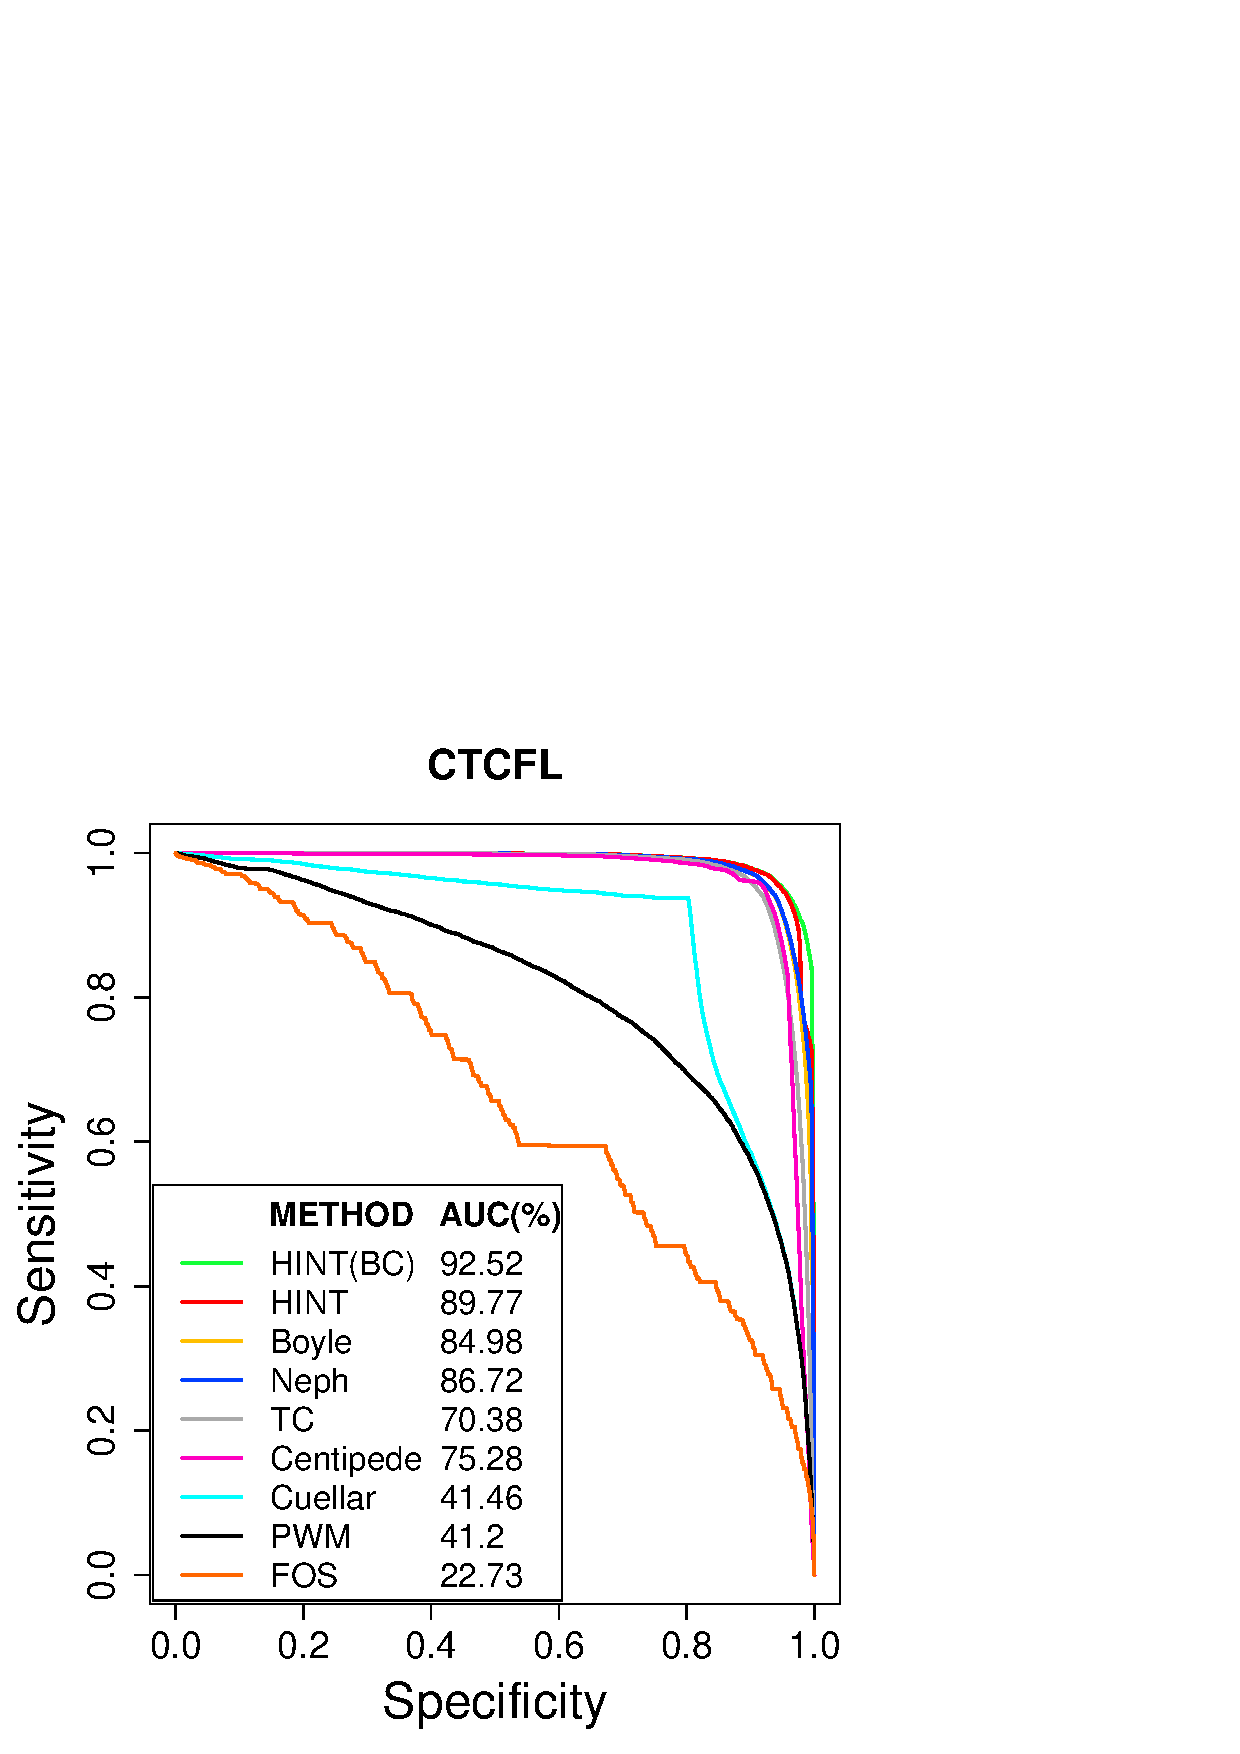
\includegraphics[width=0.49\textwidth]{CTCFL}
\caption{ROC curve created when applying the methods to data from the cell line K562. All HMM Models were trained with data from H1-hESC and K562 cell lines.}
\label{fig:roc.K562.fdr_4.10}
\end{figure}

\begin{figure}[h]
\centering
    \includegraphics[width=0.49\textwidth]{IRF1}
    \includegraphics[width=0.49\textwidth]{FOSL1}
    \includegraphics[width=0.49\textwidth]{NR2F2}
    \includegraphics[width=0.49\textwidth]{USF1}
\caption{ROC curve created when applying the methods to data from the cell line K562. All HMM Models were trained with data from H1-hESC and K562 cell lines.}
\label{fig:roc.K562.fdr_4.11}
\end{figure}

\begin{figure}[h]
\centering
    \includegraphics[width=0.49\textwidth]{THAP1}
    \includegraphics[width=0.49\textwidth]{MAFF}
    \includegraphics[width=0.49\textwidth]{CTCF}
    \includegraphics[width=0.49\textwidth]{MEF2A}
\caption{ROC curve created when applying the methods to data from the cell line K562. All HMM Models were trained with data from H1-hESC and K562 cell lines.}
\label{fig:roc.K562.fdr_4.12}
\end{figure}

\begin{figure}[h]
\centering
    \includegraphics[width=0.49\textwidth]{RFX5}
    \includegraphics[width=0.49\textwidth]{STAT2}
    \includegraphics[width=0.49\textwidth]{CCNT2}
    \includegraphics[width=0.49\textwidth]{EGATA}
\caption{ROC curve created when applying the methods to data from the cell line K562. All HMM Models were trained with data from H1-hESC and K562 cell lines.}
\label{fig:roc.K562.fdr_4.13}
\end{figure}

\begin{figure}[h]
\centering
    \includegraphics[width=0.49\textwidth]{ZNF263}
    \includegraphics[width=0.49\textwidth]{MAX}
    \includegraphics[width=0.49\textwidth]{E2F4}
    \includegraphics[width=0.49\textwidth]{STAT1}
\caption{ROC curve created when applying the methods to data from the cell line K562. All HMM Models were trained with data from H1-hESC and K562 cell lines.}
\label{fig:roc.K562.fdr_4.14}
\end{figure}

\begin{figure}[h]
\centering
    \includegraphics[width=0.49\textwidth]{SP1}
    \includegraphics[width=0.49\textwidth]{ZBTB33}
    \includegraphics[width=0.49\textwidth]{CEBPB}
    \includegraphics[width=0.49\textwidth]{GABP}
\caption{ROC curve created when applying the methods to data from the cell line K562. All HMM Models were trained with data from H1-hESC and K562 cell lines.}
\label{fig:roc.K562.fdr_4.15}
\end{figure}

\end{document}